\let\negmedspace\undefined
\let\negthickspace\undefined
\documentclass[journal,12pt,twocolumn]{IEEEtran}
\usepackage{cite}
\usepackage{amsmath,amssymb,amsfonts,amsthm}
\usepackage{algorithmic}
\usepackage{graphicx}
\usepackage{textcomp}
\usepackage{xcolor}
\usepackage{txfonts}
\usepackage{listings}
\usepackage{enumitem}
\usepackage{mathtools}
\usepackage{gensymb}
\usepackage[breaklinks=true]{hyperref}
\usepackage{tkz-euclide} % loads  TikZ and tkz-base
\usepackage{listings}
\usepackage{gvv}


\newtheorem{theorem}{Theorem}[section]
\newtheorem{problem}{Problem}
\newtheorem{proposition}{Proposition}[section]
\newtheorem{lemma}{Lemma}[section]
\newtheorem{corollary}[theorem]{Corollary}
\newtheorem{example}{Example}[section]
\newtheorem{definition}[problem]{Definition}

\newcommand{\BEQA}{\begin{eqnarray}}
\newcommand{\EEQA}{\end{eqnarray}}
\newcommand{\define}{\stackrel{\triangle}{=}}
\theoremstyle{remark}
\newtheorem{rem}{Remark}

\graphicspath{./figs/}

%\bibliographystyle{ieeetr}
\begin{document}
%

\bibliographystyle{IEEEtran}


\vspace{3cm}

\title{
%	\logo{
Assignment-2

\large{EE:1205 Signals and Systems}

Indian Institute of Technology, Hyderabad
%	}
}
\author{Kunal Thorawade

EE23BTECH11035
}	

\maketitle


\newpage

%\tableofcontents

\bigskip
 
\renewcommand{\thefigure}{\theenumi}
\renewcommand{\thetable}{\arabic{table}}
%\renewcommand{\theequation}{\theenumi}

\section{Question:}
What will Rs 500 amounts to in 10 years after its deposit in a bank which pays annual interest rate of 10$\%$ compounded annually?

\section{Solution}
\begin{table}[ht]
  \centering
  \begin{tabular}{|c|c|c|c|}
    \hline
     & \textbf{Principal} & \textbf{Interest} & \textbf{Amount} \\
    \hline
    $1^{st} Year$ & 500 &$  \dfrac{10}{100} \times 500 = 50 $ & 500 + 50 = 550 \\
    \hline
   $2^{nd} Year$ & 550 &$  \dfrac{10}{100} \times 550 = 55 $ & 550 + 55 = 605 \\
    \hline
    $3^{rd} Year$ & 605 &$  \dfrac{10}{100} \times 605 = 60.5 $ & 605 + 60.5 = 665.5 \\
    \hline
  \end{tabular}
  \vspace{2mm}
  \caption{GP Table}
  \label{tab:mytable}
\end{table}

From above table:

The series is 550, 605, 665.5...

\begin{table}[ht]
    \centering
    \begin{tabular}{|c|c|}
        \hline
        Parameter & Value \\
        \hline
        First term of AP (x(0)) & 5 \\
        \hline
        Common difference (d) & 1.75 \\
        \hline
        $n^{th}$ term of AP (x(n)) & 20 \\
        \hline
    \end{tabular}
    \vspace{2mm}
    \caption{Parameter List}
    \label{tab:simple}
\end{table}

From \tabref{tab:11.9.3.31}:

The Z-transform of a sequence $x(n)$ is given by:

\begin{align}
    X(Z) = \frac{550}{1 - (1.1)z^{-1}} ; |z| > 1.1
\end{align}

\begin{figure}
    \centering
    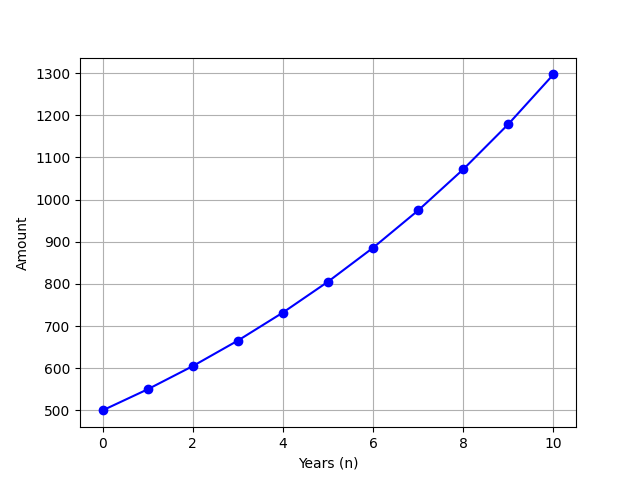
\includegraphics[width = 8cm]{figs/fig1.png}
    \caption{Plot of $x(n) = 550(1.1)^n$}
    \label{fig:enter-label}
\end{figure}
\end{document}
